\chapter{Additional Files and Schematics}
\label{ch_appendixa}

%Add any information here that you would like to have in your project but is not necessary in the main
%text. Remember to refer to it in the main text. Separate your appendices based on what they are for
%example. Equation derivations in Appendix A and code in Appendix B etc.

\lstinputlisting[caption={Optimized Goertzel Algorithm - Octave Function\label{lst:optimized_goertzel_algorithm}}]{../goertzel/hc_calculate_goertzel.m}

\lstinputlisting[caption={Frequency Response Test - Octave Script\label{lst:frequency_response_script}}]{../goertzel/test_goertzel.m}

\begin{figure}[H]
	\centering
	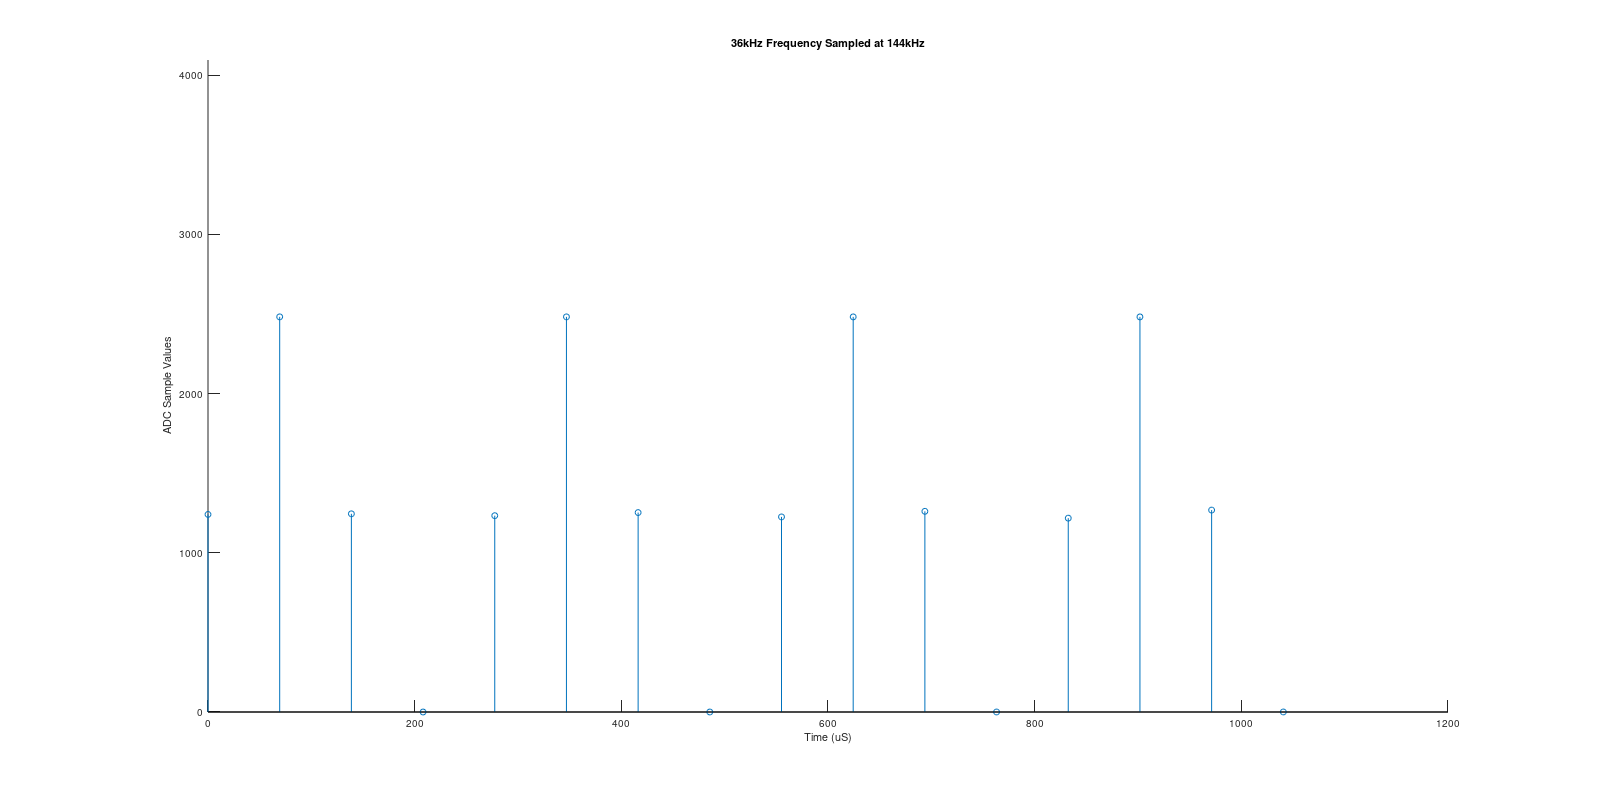
\includegraphics[width=\linewidth]{figures/results/36khz_frequency.png}
	\caption{Plot of sampled 36kHz sinusoid}
	\label{fig:sampled_36khz_sinusoid}
\end{figure}

\begin{figure}[H]
	\centering
	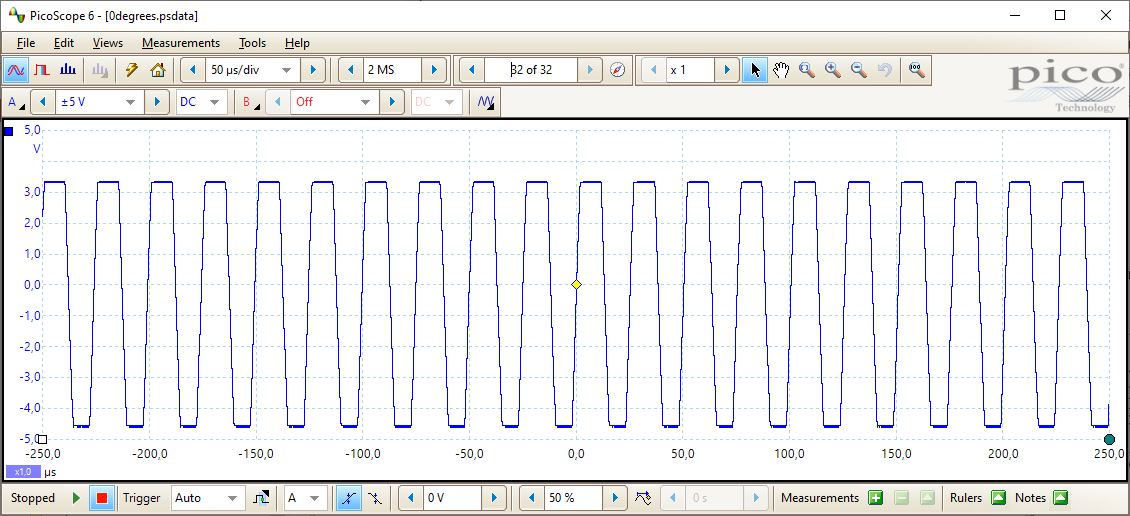
\includegraphics[width=\linewidth]{figures/appendix/photodiode_0degrees.JPG}
	\caption{Output of photodiode module prior to full saturation}
	\label{fig:begin_saturation_of_photodiode}
\end{figure}

\begin{lstlisting}[style=cstyle, caption=Timer Interrupt Handler Implementation\label{lst:manchester_generate_interrupt_routine}]
	if(htim == &htim17){
	
		if(bit_index == bit_num_transmit){
			HAL_GPIO_WritePin(GPIOB, GPIO_PIN_10, GPIO_PIN_RESET);
			manchester_timeout_counter++;
		
		}else if(fire_in_progress){
			if(bit_period ^ ((~bit_stream >> bit_index) & 1)){
				HAL_GPIO_WritePin(GPIOB, GPIO_PIN_10, GPIO_PIN_SET);
			}else{
				HAL_GPIO_WritePin(GPIOB, GPIO_PIN_10, GPIO_PIN_RESET);
			}
			
		bit_index += bit_period;
		bit_period = !bit_period;
		
		}
		
		if(manchester_timeout_counter == TIMEOUT_BIT_PERIODS){
			fire_in_progress = 0;
			HAL_TIM_Base_Stop_IT(&htim17);
		}
	}
\end{lstlisting}



\begin{lstlisting}[style=cstyle, caption=Generate Manchester Function Implementation\label{lst:generate_manchester_implementation}]
	generate_manchester(uint32_t buffer, uint8_t num_bits){
		//generates a manchester waveform on pin PB10 according to the bits in the buffer
		
		while(fire_in_progress == 1); //wait for any current transmission to end
		
		HAL_TIM_Base_Stop_IT(&htim17); //stop the timer during setup
		fire_in_progress = 1; //set fire in progress to indicate
		bit_stream = buffer & ((1 << num_bits) - 1); //set all bits higher than number of bits to send to zero
		bit_num_transmit = num_bits; //set the final index based on number of bits to transmit
		bit_index = 0; //reset index pointer to beginning of buffer
		bit_period = 0; //reset the bit period tracker
		manchester_timeout_counter = 0; // reset the timer out counter
		HAL_TIM_Base_Start_IT(&htim17); //begin the timer (starts the transmission process)
	}
\end{lstlisting}


\begin{lstlisting}[style=cstyle, caption=Manchester Decoding - State Machine Implemenation\label{lst:decode_manchester_implementation}]
static uint16_t manchester_decode(uint32_t* edges, int num_edges){

	uint32_t decoding_buffer;
	enum decoding_states state = md_reset;
	int index = 0;
	int error_flag;
	int short_period;
	
	for (int edge = 0; edge < num_edges; edge++){
		error_flag = 0;
		short_period = 0;
		
		if (edges[edge] < THRESHOLD_TICKS){
			short_period = 1;
		}else if (edges[edge] > BITMISS_TICKS){
			error_flag = 1;
		}
		
		switch (state){
		case md_reset:
			index = 1;
			decoding_buffer = 1;
			state = md_moo;
			break;
		
		case md_moo:
			if (short_period){
				state = md_soo;
			}else{
				state = md_moz;
				decoding_buffer &= ~(1 << index++);
			}
			break;
		
		case md_moz:
			if (short_period){
				state = md_soz;
			}else{
				state = md_moo;
				decoding_buffer |= 1 << index++;
			}
			break;
		
		case md_soo:
			if (short_period){
				state = md_moo;
				decoding_buffer |= 1 << index++;
			}else{
				//Error has occurred
				error_flag = 1;
			}
			break;
		
		case md_soz:
			if (short_period){
				state = md_moz;
				decoding_buffer &= ~(1 << index++);
			}else{
				//Error has occurred
				error_flag = 1;
			}
			break;
		}
		
		if(error_flag){
			break;
		}
	
	}
	
	error_flag |= (index != 18);//check that 18 bits have been decoded or if earlier error was detected
	
	if(error_flag){
		decoding_buffer = 1 << 17; //all zeros with 16th data bit a '1' indicates an error
	}
	
	if(!error_flag){
		print_lcd(decoding_buffer);
	}
	return (uint16_t) (decoding_buffer >> 2);

}
\end{lstlisting}